% !Mode:: "TeX:UTF-8"

\chapter{GPSA系统分析}
本章对GPSA系统进行高效性、可行性与稳定性分析。首先从Actor-BSP模型入手解释GPSA的正确性和高效性,然后从IO角度对GPSA在单机系统上的可行性进行说明,接着从容错性的角度介绍GPSA的稳定性。最后,通过如何在GPSA系统上实现常用的图应用进行举例说明。

\section{Actor-BSP模型分析}
首先,Actor-BSP模型与以往的以顶点为中心的模型的异同使得Actor-BSP模型具有类似的语义,从而保证模型的正确性。Actor-BSP模型是以Actor角色作为中心的,但是新模型并没有完全消除以顶点为中心的概念。而仅仅是对其进行淡化,使得在顶点上的计算转移到角色上进行,同时能够兼顾顶点状态的更新而无需关注顶点和角色之间的强制的依赖关系。另外,Actor角色还分担了传统意义上线程的执行者的角色。以往线程负责对顶点进行遍历并调用顶点上的消息处理函数,在新模型中则是Actor角色负责遍历顶点并调用提供给Actor的消息处理函数。

其次,Actor-BSP模型将计算过程和消息分发过程分离使得GPSA能够获得性能提升。在以顶点为中心的图计算中,对于顶点而言,其计算过程和消息发送过程是紧密相关,不经过对顶点的状态信息进行计算就不能发送顶点的更新消息。所以,此时顶点的计算过程和消息发送过程是严格意义上的顺序执行。对于BSP的应用而言,执行时间最长的任务决定整体的效率。Actor-BSP模型是在执行过程上完全异步计算的模型,计算过程与消息分发过程想分离,使得两个过程可以在一定程度上并行执行。在Actor-BSP模型中,Actor分为两种类型:负责消息分发过程的分发Actor和负责计算过程的计算Actor。得益于分发Actor和计算Actor之间的松耦合设计,两者之间的映射关系变得相当的灵活,缩短BSP模型在垂直方向上的执行时间,提高处理效率。

最后,Actor-BSP模型的轻量级与高并发。Actor并发模型本身就是一种轻量级的高并发的编程模型。Actor擅长处理消息,不同的Actor之间通过邮箱通讯,摒弃基于内存共享并发模型的同步和锁等概念。



其次,分发Actor 和 计算Actor 组成了生产者和消费者模型,当消息到达计算Actor之后,该actor会被调度执行,处理消息,从而无需保存这些消息,避免将消息进行缓存的IO开销。

\section{IO分析}

单机系统上的图处理系统不仅仅需要进行大量的计算,与此同时还会涉及大量的IO操作。以往的图处理系统中,除了需要在更新顶点状态信息的时候需要写入大量的数据,还需要缓存大量的消息以供系统在下一个超级步进行计算。所以,整体而言需要写入磁盘的数据非常多,IO开销非常巨大。由于在单机系统中,大量的IO操作会成为系统的主要瓶颈,所以在其他系统都是从优化IO问题着手,通过避免图数据的随机访问问题,批量写入大块数据来解决IO问题。

与其他单机上图处理系统不同,GPSA没有刻意去避免随机访问的问题,GPSA首先对图数据在新模型下的访问行为进行详细的分析和讨论,然后根据访问行为的不同,将图数据分为两部分。一部分支持随机访问,通过内存映射的方式使之常驻内存;另外一部分则不支持随机访问,保存于磁盘通过顺序访问的方式进行数据的读取操作。其次,GPSA最大的IO优势之一:GPSA无需缓存大量的消息到磁盘中。在GPSA中,Actor分为两种不同的类型:分发Actor和计算Actor。分发Actor负责消息的产生和发送工作;计算Actor则负责消息的处理和顶点的状态信息更新。从Actor的角度分析,分发Actor 和 计算Actor 组成了生产者和消费者模型,当消息到达计算Actor之后,受到消息驱动的计算过程便会开始执行从而无需保存这些消息,避免将消息进行缓存的IO巨大开销。

\section{容错性分析}

容错性是系统安全稳定运行的重要保证。在GraphChi和X-Stream中,实现容错性非常困难。这是因为它们需要保存大量的数据信息和图处理的中间结果。但是,系统崩溃往往是一刹那的事情,在短时间内完成大量数据的信息保存时非常困难的。

得益于GPSA将图数据的区分对待,容错性得到很好的保证。本系统中发生改变的数据只有顶点的状态信息,并且无需保存大量的消息,所以只要能够在系统崩溃时找到一个保存了完整图顶点状态信息的时间点就能从改时间点对系统进行恢复。在本系统的设计中,顶点的状态信息是以“Two-Column”的方式保存在内存映射文件中的,同时计算Actor和分发Actor分别访问不同数据列,并且分发Actor只能读取数据,而只有计算Actor才能写入数据。也就意味着,分发Actor所读取的数据列的结果就是上一个超级步的图顶点状态信息的完整备份。

如图 \ref{fig:ft}所示,如果系统在超级步1崩溃,此时顶点状态信息如图\ref{fig:ft:ft}所示。在超级步1,右边是分发列,左边是计算列。所以右边的分发列就是超级步0完成之后的正确结果。系统可以从该列进行数据恢复操作。

\begin{figure}[htbp]
  \centering
  \subfigure[正常时的执行情况]{\label{fig:ft:vu}
                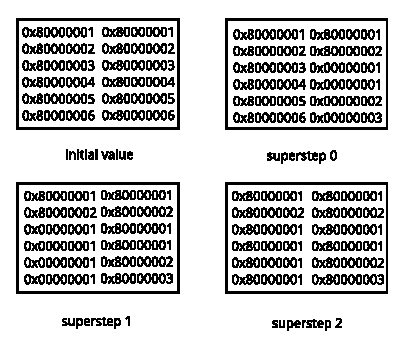
\includegraphics[width=0.4\textwidth]{myfigures/valueupdating.eps}}
  \subfigure[崩溃时的执行情况]{\label{fig:ft:ft}
                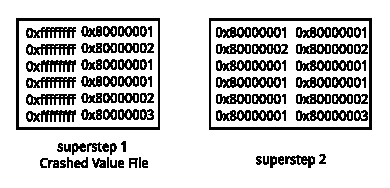
\includegraphics[width=0.4\textwidth]{myfigures/faulttolerant.eps}}
  \caption{容错性}\label{fig:ft}
\vspace{\baselineskip}
\end{figure}




\section{应用示例}
在GPSA的框架上实现应用会非常简单,一般情况下只需要实现\textit{Handler}接口,在该接口必须要实现的函数有两个:\textnormal{init(sequence)}和\textnormal{compute(val,msgVal,args)}。其中,\textnormal{init}函数主要用于初始化顶点的状态信息,而compute方法则用于在计算Actor处理消息时进行调用。除此之外,还有一些可选函数,例如消息生成函数、更新判定等,如果不实现这些可选函数,则会以默认方式进行计算。例如,若不实现消息生成函数,则默认将顶点的最新状态打包进消息中进行发送。

\subsection{PageRank}
PageRank是著名的网页排名算法。在GPSA中实现该算法,需要实现\textit{Handler}接口,将顶点的初始值初始化为1.0,然后当计算Actor接收到消息进行计算时,需要对这些消息进行累加,如算法\ref{al:pr}所示。
\begin{algorithm}
{
{
\renewcommand\baselinestretch{1.5}\selectfont %控制行距

\caption{PageRank}
\label{al:pr}
\begin{algorithmic}[1]
\REQUIRE ~\\
	$val,msgVal,args$
\ENSURE ~\\
	$newVal$
\IF{$args[0]$}
	 \RETURN $ 0.15f$
\ENDIF
\RETURN $0.85*msgVal + vertexVal$

\end{algorithmic}
}
\par}
\end{algorithm}

\subsection{BFS}
BFS是对图进行广度遍历的算法。在GPSA中实现该算法则需要指定起始遍历的顶点,起始顶点的值初始化为0,其他顶点初始化为无穷大,通过发送消息并对消息进行计算可以得到某一个顶点在广度遍历中在整个图中的遍历层次。对于一个顶点而言,假如\textit{V}所处的层次为n,那么它的出边的顶点的层次在没有其他干扰情况下(例如,这些顶点同时也是层次为n-1的顶点的出边目的顶点)是n+1。否则,可以通过比较他的目的顶点的层次与它的消息中的新层次,最小的那个即为其在广度遍历算法中的层次。由于无法保证消息的发送和接收顺序,所以在计算函数中通过比较消息的值的层次的大小,并将值最小的消息加1之后作为返回值,具体实现如算法\ref{al:bfs}。
\begin{algorithm}
{
{
\renewcommand\baselinestretch{1.5}\selectfont %控制行距

\caption{Breadth First Search}
\label{al:bfs}
\begin{algorithmic}[1]
\REQUIRE ~\\
	$val,msgVal,args$
\ENSURE ~\\
	$newVal$
\IF{$msgVal < val$}
	 \RETURN $ msgVal + 1$
\ENDIF
\RETURN $val$

\end{algorithmic}
}
\par}
\end{algorithm}
\subsection{CC}
联通分量的实现过程与广度搜索类似,但是在初始化的时候,将所有顶点的值初始化为其自身\textit{id},然后在计算函数中通过比较两者的\textit{id}的大小,选择返回较小值。这样,计算完成
之后,处在同一个连通分量中的顶点拥有相同的\textit{id},具体实现如算法\ref{al:cc}所示。
\begin{algorithm}
{
{
\renewcommand\baselinestretch{1.5}\selectfont %控制行距

\caption{CC}
\label{al:cc}
\begin{algorithmic}[1]
\REQUIRE ~\\
	$val,msgVal,args$
\ENSURE ~\\
	$newVal$
\IF{$msgVal < val$}
	 \RETURN $ msgVal$
\ENDIF
\RETURN $val$

\end{algorithmic}
}
\par}
\end{algorithm}

\subsection{小结}


本章是GPSA系统的分析部分,在前面几章对图处理技术和GPSA系统的设计与实现介绍的基础上,进一步对GPSA系统进行了多个方面的分析。主要从系统整体的可行性、效率、稳定性和便捷性对系统进行分析。首先,对GPSA的计算模型从模型语义、结构和并发三个角度进行分析,解释GPSA高效的原因;其次,对GPSA的将图分为两部分,从而实现两种不同IO操作方式进行说明,并且指出GPSA无需缓存大量消息;接下来,对GPSA的“Two-Column”存储方式的容错性进行介绍,证明GPSA系统的稳定性;最后,通过举例说明在GPSA系统上开发的便捷性。



